\documentclass{beamer}

\mode<presentation>
{
  \usetheme{CambridgeUS}
  \setbeamercovered{transparent}
}

\usepackage[english]{babel}
\usepackage[latin1]{inputenc}
\usepackage{times}
\usepackage[T1]{fontenc} 
% Or whatever. Note that the encoding and the font should match. If T1
% does not look nice, try deleting the line with the fontenc.
\usepackage{amsmath}

\newcommand{\linespace}{\vskip 0.25cm}

\definecolor{MyForestGreen}{rgb}{0,0.7,0} 
\newcommand{\tableemph}[1]{{#1}}
\newcommand{\tablewin}[1]{\tableemph{#1}}
\newcommand{\tablemid}[1]{\tableemph{#1}}
\newcommand{\tablelose}[1]{\tableemph{#1}}

\definecolor{MyLightGray}{rgb}{0.6,0.6,0.6}
\newcommand{\tabletie}[1]{\color{MyLightGray} {#1}}

% The text in square brackets is the short version of your title and will be used in the
% header/footer depending on your theme.
\title[Test-First vs. Test-Last Testing]{An Exploration into the Current State \\ of Test-First vs. Test-Last Testing}

% Sub-titles are optional - uncomment and edit the next line if you want one.
% \subtitle{Why does sub-tree crossover work?} 

% The text in square brackets is the short version of your name(s) and will be used in the
% header/footer depending on your theme.
\author[Thomas]{Christopher Morris Thomas}

% The text in square brackets is the short version of your institution and will be used in the
% header/footer depending on your theme.
\institute[U of Minn, Morris]
{
  Division of Science and Mathematics \\
  University of Minnesota, Morris \\
  Morris, Minnesota, USA
}

% The text in square brackets is the short version of the date if you need that.
\date[2013 Fall Senior Seminar] % (optional)
{2013 Fall Senior Seminar}

% Delete this, if you do not want the table of contents to pop up at
% the beginning of each subsection:
\AtBeginSection[]
{
  \begin{frame}<beamer>
    \frametitle{Outline}
    \tableofcontents[currentsection, hideothersubsections]
  \end{frame}
}

\begin{document}

\begin{frame}
  \titlepage
\end{frame}

% For a 20-25 minute senior seminar talk you probably want something like:
% - Two or three major sections (other than the summary).
% - At *most* three subsections per section.
% - Talk about 30s to 2min per frame. So there should probably be between
%   15 and 30 frames, all told.

\section*{Overview}

\subsection*{Outline}

\begin{frame}
  \frametitle{Outline}
  \tableofcontents[hideallsubsections]
\end{frame}

\section[Background]{Background}
\subsection{What is testing?}
\begin{frame}
\frametitle{Why Do we Care about testing methods?}
In 2007, a study it was found that businesses spent at least 50\% of their production costs on product verification and testing.
\linespace
\linespace
Because of this, software businesses are constantly looking to optimize their testing practices in an attempt to reduce costs.
\end{frame}

\begin{frame}
\frametitle{Software Testing Defined}
Software testing is a branch of software
engineering that uses various practices to:
\begin{itemize}
\item identify potential malfunctions in code
\item demonstrate functionality of software
\end{itemize}
\linespace
Testing is usually either done manually or automatically using test code.
\end{frame}

\subsection{Test-Last Testing and Waterfall Development}

\begin{frame}
\frametitle{Waterfall Development}
\begin{columns}
\begin{column}{.4\textwidth}
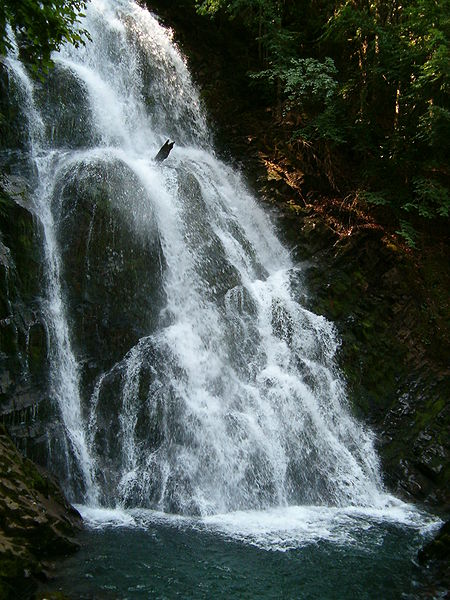
\includegraphics[scale=.25]{Waterfall.JPG}
\\
\only{\tiny Wikipedia Commons \\
{\url{commons.wikimedia.org/wiki/File:Waterfall_near_Brienzersee.jpg}}}
\end{column}
\begin{column}{0.6\textwidth}
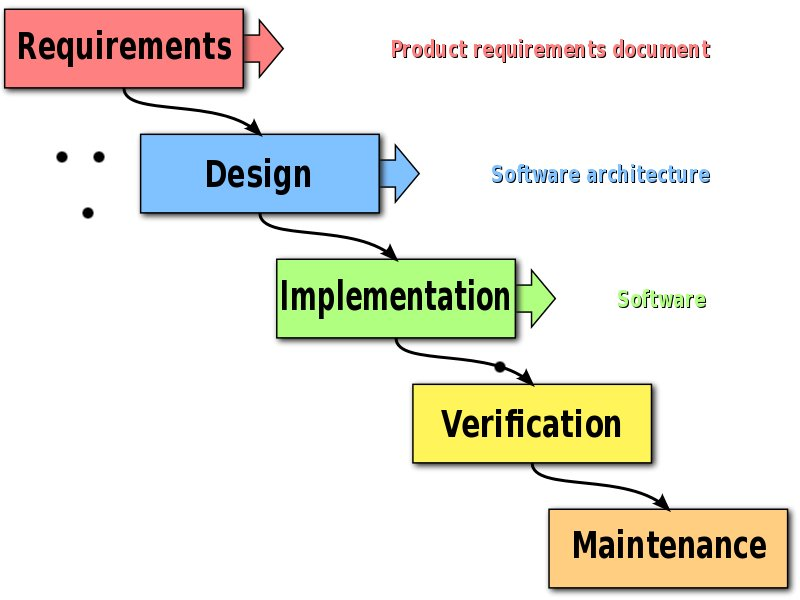
\includegraphics[scale=.3]{Waterfall_model.jpg}
\\
\only{\tiny Wikipedia \\
{\url{en.wikipedia.org/wiki/File:Waterfall development_model.svg} }}
\end{column}
\end{columns}
\end{frame}

\begin{frame}
\frametitle{Test-Last Testing}
Test-last testing is:
\begin{itemize}
\linespace
\item Writing tests after the code
\linespace
\item Used in waterfall development
\linespace
\item Considered the ``conventional testing method"
\end{itemize}
\end{frame}

\subsection{Test-First Testing and Test Driven Development}

\begin{frame}
\frametitle{Agile Software Development}
Agile development was developed in response to criticisms of waterfall methods.

\linespace

Some common traits of agile development:
\begin{itemize}
\item Time boxed iterations
\item working sub-products
\item Customer communication
\item Test driven development
\end{itemize}
\end{frame}

\begin{frame}
\frametitle{Test-First Testing}
Test-first testing is:
\begin{itemize}
\linespace
\item writing automated tests before the code is written
\linespace
\item often used to define code functionality
\linespace
\item usually used as part of a development model 
\end{itemize}
\end{frame}

\begin{frame}
\frametitle{Test Driven Development}
Test driven development (TDD) is the most well known and used test-first development model.  Currently, TDD refers to a wide variety of different test-first methods that are similar to the original TDD method as defined by Kent Beck.
\linespace
The original TDD method consists of three steps that are repeated until the program is complete:
\begin{itemize}
\item Write a new failing test
\item Write code to make tests pass
\item Optimize your new code
\end{itemize}
\linespace

\end{frame}

\section[Comparison of Testing Methods]{Comparison Between Test-First and Test-Last Testing}

\subsection{Measuring Test Methods}

\begin{frame}
\frametitle{Measuring Test Methods}
When it comes to comparing two test methods there is no one attribute that proves one method is superior to another.

\linespace

While there are many attributes that can be used to compare testing methods, I focused on three attributes:
\begin{itemize}
\item code coverage
\item total development time
\item code correctness
\end{itemize}
\end{frame}

\subsection{Current Data}

\begin{frame}
\frametitle{Article review by Kollanus}
In 2010, Kollanus reviewed 40 different articles that provided empirical evidence comparing TDD to test-last development methods.
\linespace
\linespace
\linespace
In the review Kollanus found that TDD methods:
\begin{itemize}
\item potentially had better code correctness
\item potentially had longer development times
\item suggested by one study increase code coverage
\end{itemize}
\end{frame}

\begin{frame}
\frametitle{Lemos et al Study Setup}
In 2012, Lemos et al preformed an experiment comparing test-first and test-last testing with auxiliary functions (10-200 lines of code).

\linespace

In the study, Lemos had third year computer science students with basic test-first and test-last knowledge solve coding problems using test-first and test-last development methodologies.

\linespace
\end{frame}

\begin{frame}
\frametitle{Lemos et al Results}
After the study was completed Lemos found that test-first testing:
	\begin{itemize}
	\linespace
		\item produced 40\% more code coverage than test-last testing
	\linespace
		\item took 12\% longer to implement than test-last testing
	\linespace 
		\item did not increase code correctness
	\end{itemize}
\end{frame}

\subsection{Discussion}

\begin{frame}
\frametitle{Contradictory Studies}
One large problem currently in the test-first vs test-last debate is that many studies contradict each other.

\linespace

Although no one currently knows exactly why these contradictions occur, a few theories exist.  Three potential problems in current TDD research that could produce contradictions are:
\begin{itemize}
\item method difficulty
\item lack of TDD method documentation
\item TDD conformance issue
\end{itemize}
\end{frame}

\begin{frame}
\frametitle{Method Difficulty}
Results from an opinion study by Janzen et al:
\begin{columns}
\begin{column}{.5\textwidth}
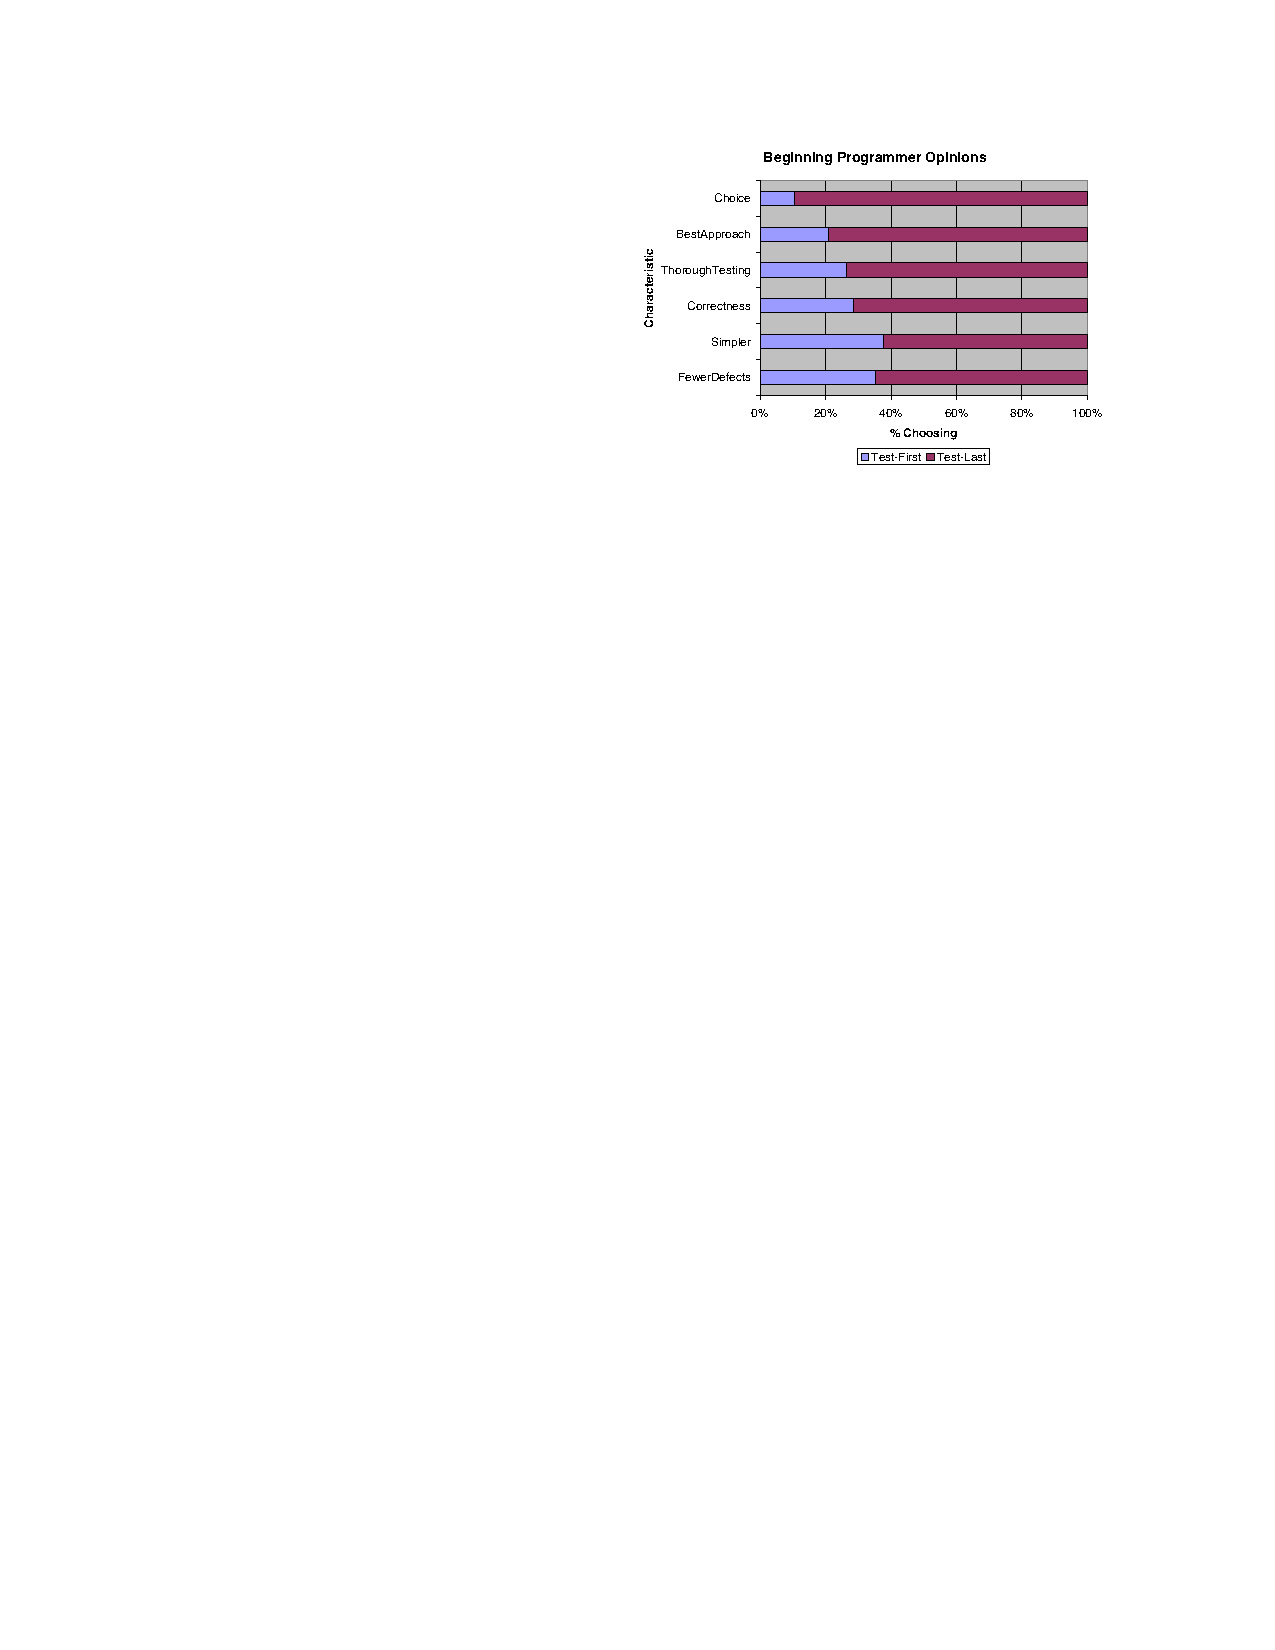
\includegraphics[scale=.75]{janzengraph1.pdf}
\\
\end{column}
\begin{column}{.5\textwidth}
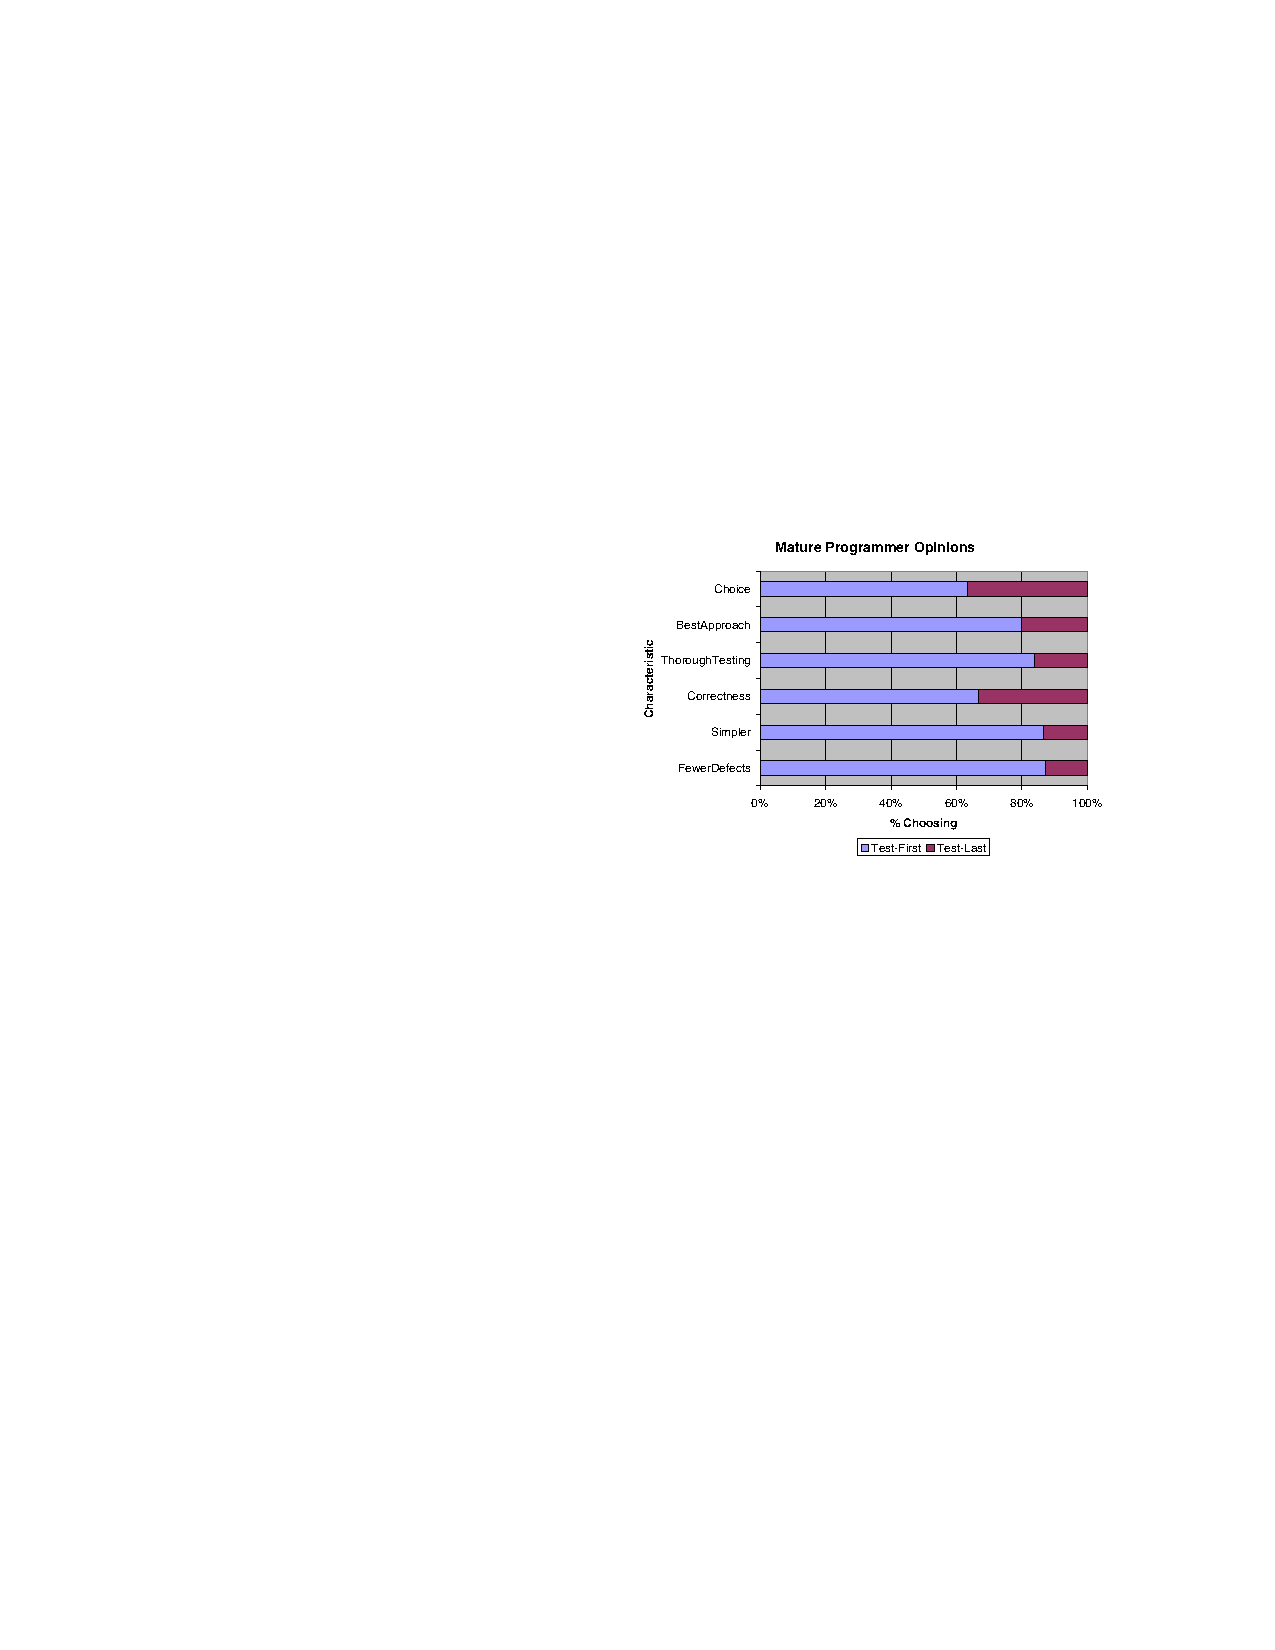
\includegraphics[scale=.75]{janzengraph2.pdf}
\\
\end{column}
\end{columns}
\end{frame}

\begin{frame}
\frametitle{Conclusions}
Due to current issues in contradictory data it is hard to make solid conclusions.
\linespace
That being said some strong trends were noticed:
\begin{itemize}
\item  test-first testing takes at least as much time as test-last testing
\item test-first testing tends to increase code coverage
\item test-first testing has at least the same code correctness as test-last testing
\item test-first testing is potentially more difficult then test-last testing
\end{itemize}
\end{frame}

\section[Different Implementations of Test-First]{Different ways of Implementing Test-First Testing} 

\subsection{The challenges of Test Driven Development}

\begin{frame}
\frametitle{Difficulty of TDD}
Most the data for test-first testing comes from studies using TDD.  This means that the results have a potential to reflect properties of TDD and not test-first testing.
\linespace
\linespace
Although all the trends have this potential issue.  The most worrisome data point is method difficulty.  This is because many articles noted that TDD can be a hard to implement for reasons other then test-first testing.
\end{frame}

\begin{frame}
\frametitle{Difficulty of TDD Cont.}
In a survey given to participants of a series of TDD experiments it was noted that:
\begin{itemize}
\item 56\% of participants said they had difficulty adapting to the TDD mindset
\item 23\% of participants said that lack of upfront design was found to be a hinderence
\end{itemize}
\linespace
\linespace

Another survey, given online, found that \textbf{25\% of TDD programmers admitted to frequently or always making mistakes in following the steps of TDD}.  Some of these mistakes include:
\begin{itemize}
\item writing tests that are too complex for effective TDD
\item forgetting to optimize their new code
\end{itemize}
\end{frame}

\begin{frame}
\frametitle{TDD Difficulty Cont. 2}
Results from the opinion study by Janzen et al:
\begin{columns}
\begin{column}{.5\textwidth}
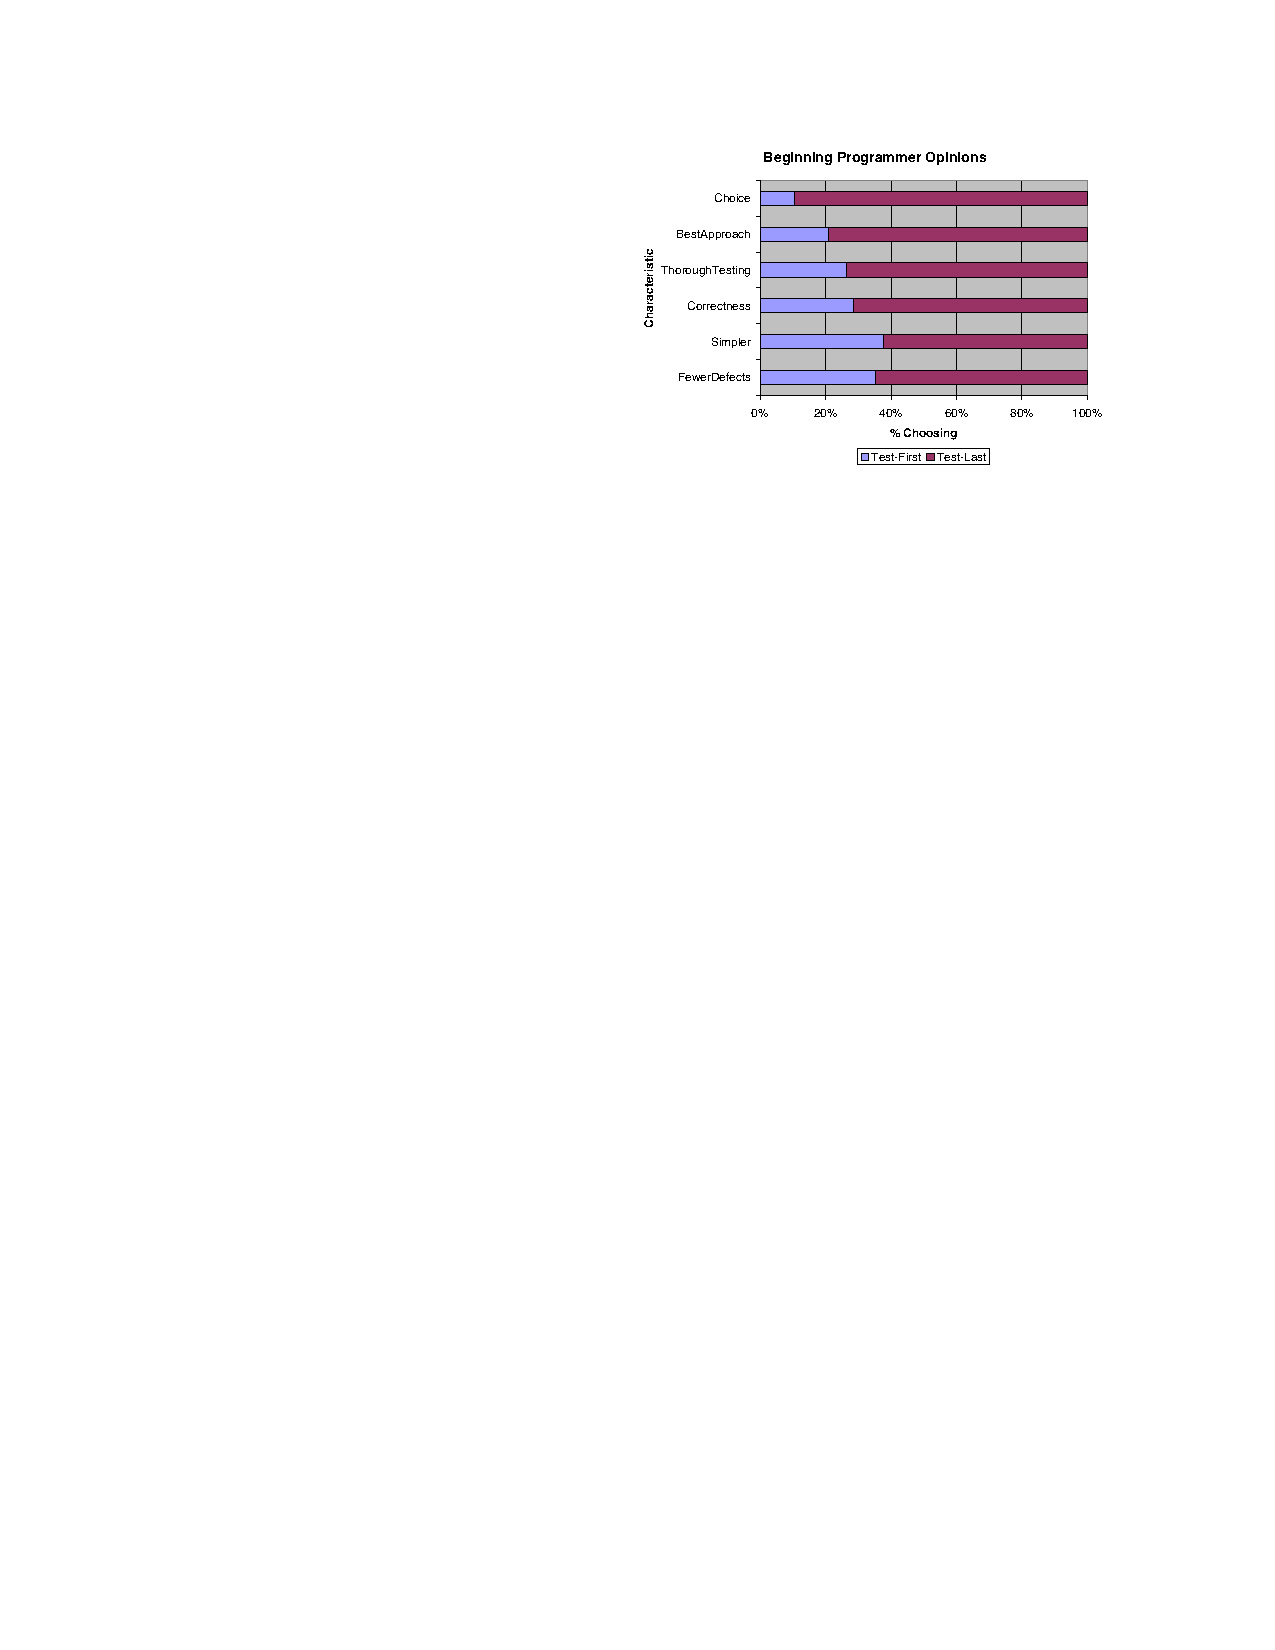
\includegraphics[scale=.75]{janzengraph1.pdf}
\\
\end{column}
\begin{column}{.5\textwidth}
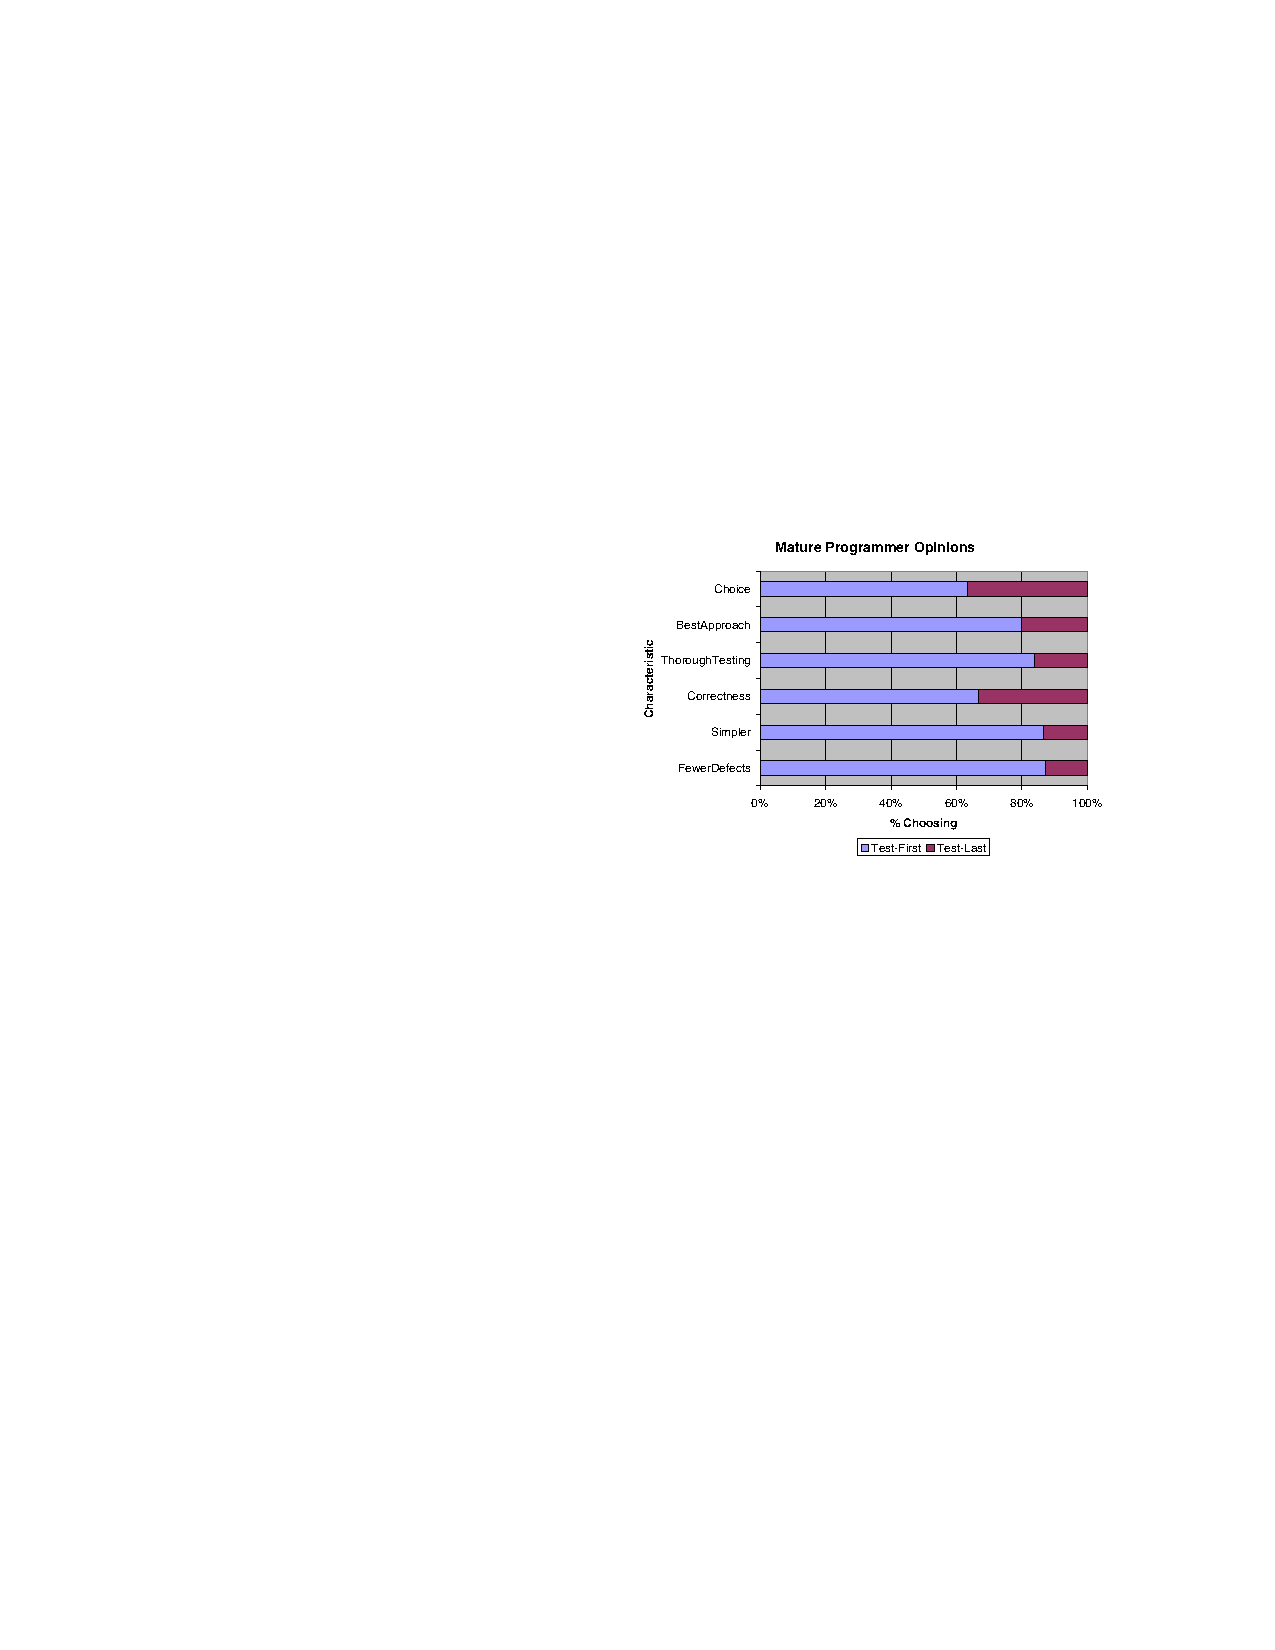
\includegraphics[scale=.75]{janzengraph2.pdf}
\\
\end{column}
\end{columns}
\end{frame}

\subsection{Things to Take Away From this Presentation}
\begin{frame}
\frametitle{Things to Take Away From this Presentation}
\begin{itemize}
\item currently testing can be divided into test-first and test-last testing
\item test-first testing tends to be favored in Agile Development
\item test-last testing tends to be favored in Waterfall Development
\item Current data on comparing test-first to test-last testing tends to produce contradictory results over multiple studies, though a few main trends in the data exist
\item TDD may not be the optimal way to preform test-first testing.
\end{itemize}

\end{frame}


\end{document}


